\documentclass[aspectratio=169,utf8,t]{beamer}

% Idioma e Codificacao
\usepackage[brazilian]{babel}
\usepackage{booktabs}
\usepackage{array}
\usepackage{listings}
\usepackage{amsmath}
\usepackage{amssymb}
\usepackage{graphicx}

% Carrega o Tema Modelo dos Scouts (Widescreen 16:9, Nunito Sans)
\usetheme{scouts}

% Configuracao para Codigo-Fonte (Python / JSON / Bash)
\lstset{
    basicstyle=\ttfamily\scriptsize,
    keywordstyle=\bfseries\color{ScoutNavy},
    stringstyle=\color{ScoutGreen},
    commentstyle=\itshape\color{gray},
    backgroundcolor=\color{black!3},
    frame=single,
    rulecolor=\color{black!15},
    breaklines=true,
    showstringspaces=false,
    tabsize=2
}

% Metadados Institucionais
\author{Prof. Me. Reginaldo Fernandes}
\institute{Instituto Federal do Ceará -- Campus Tauá \\ Tecnologia em Análise e Desenvolvimento de Sistemas}
\title{Bancos de Dados Não-Relacionais}
\subtitle{Aula 02: Teoremas CAP \& PACELC e Paradigma BASE vs ACID}
\date{06 de Outubro de 2026}

\begin{document}

% ------------------------------------------------------------------------------
% Capa da Apresentacao
% ------------------------------------------------------------------------------
\changecolours[inverse]{ScoutGreen}
\frame[plain]{\titlepage}

% ------------------------------------------------------------------------------
% Sumario Executivo da Aula
% ------------------------------------------------------------------------------
\changecolours{ScoutGreen}
\begin{frame}{Agenda do Encontro}
  \vspace{0.4cm}
  \tableofcontents
\end{frame}

% ------------------------------------------------------------------------------
% Modulos da Aula
% ------------------------------------------------------------------------------
\changecolours{ScoutNavy}
\section{O Dilema dos Sistemas Distribuídos}

% ------------------------------------------------------------------------------
\twocolframe[title={De um Único Servidor para Clusters Distribuídos},leftcol=7cm,rightcol=7cm]{%
  \alert{O Mundo Relacional Clássico (Aula 01)}\par
  \itemseps[topsepi=2mm,itemsepi=3mm,labelsep=2mm,leftmargini=4mm]
  \begin{itemize}
    \item Na Aula 01, vimos que bancos relacionais operam tradicionalmente sob \textbf{Escala Vertical (Scale-Up)}.
    \item Todas as leituras e escritas ocorrem na \textbf{mesma CPU e na mesma memória RAM}.
    \item A consistência é trivial: uma única máquina centralizada é dona da verdade absoluta.
    \item \textbf{Problema:} Teto físico de hardware e custo exponencial para sustentar Big Data.
  \end{itemize}
}{%
  \alert{A Realidade NoSQL: O Cluster Distribuído}\par
  \itemseps[topsepi=2mm,itemsepi=3mm,labelsep=2mm,leftmargini=4mm]
  \begin{itemize}
    \item Para escalar horizontalmente (\textbf{Scale-Out}), particionamos dados entre dezenas ou centenas de servidores.
    \item \textbf{Novo Desafio Arquitetural:} Os nós precisam se comunicar continuamente através de placas de rede e roteadores.
    \item \textbf{Falhas Parciais:} Diferente de um único servidor que cai por inteiro, no cluster um nó pode falhar enquanto outros continuam ativos.
  \end{itemize}
}

% ------------------------------------------------------------------------------
\twocolframe[title={As 8 Falácias da Computação Distribuída},leftcol=7cm,rightcol=7cm]{%
  \alert{Deutsch \& Gosling (Sun Microsystems, 1994)}\par
  \itemseps[topsepi=2mm,itemsepi=2.5mm,labelsep=2mm,leftmargini=4mm]
  \begin{itemize}
    \item Todo desenvolvedor júnior comete suposições ingênuas que quebram em produção:
    \item 1. \textit{``A rede é confiável.''} (Falso: fibras rompem, switches travam).
    \item 2. \textit{``A latência é zero.''} (Falso: viajar entre SP e Fortaleza consome tempo físico).
    \item 3. \textit{``A largura de banda é infinita.''}
    \item 4. \textit{``A rede é segura.''}
  \end{itemize}
}{%
  \alert{As Falácias Estruturais}\par
  \itemseps[topsepi=2mm,itemsepi=2.5mm,labelsep=2mm,leftmargini=4mm]
  \begin{itemize}
    \item 5. \textit{``A topologia da rede nunca muda.''} (Nós entram e saem).
    \item 6. \textit{``Existe apenas um administrador.''}
    \item 7. \textit{``O custo de transporte é zero.''}
    \item 8. \textit{``A rede é homogênea.''}
    \item \textbf{Impacto nos Bancos:} Como garantir que um cliente no Ceará e outro em São Paulo vejam o mesmo saldo ao mesmo tempo?
  \end{itemize}
}

% ------------------------------------------------------------------------------
\twocolframe[title={Cenário Prático: A Black Friday e o Saldo Bancário},leftcol=7cm,rightcol=7cm]{%
  \alert{O Drama do Arquiteto de Software}\par
  \itemseps[topsepi=2mm,itemsepi=3mm,labelsep=2mm,leftmargini=4mm]
  \begin{itemize}
    \item Imagine as 00:00 da Black Friday: 100.000 requisições por segundo.
    \item Um cliente em Tauá possui R\$ 500,00 na conta e tenta fazer um PIX de R\$ 500,00 simultaneamente a uma compra no cartão.
    \item Ao mesmo tempo, um rompimento de fibra óptica isola o data center de Fortaleza do data center de São Paulo.
  \end{itemize}
}{%
  \alert{A Encruzilhada Operacional}\par
  \itemseps[topsepi=2mm,itemsepi=3mm,labelsep=2mm,leftmargini=4mm]
  \begin{itemize}
    \item \textbf{Opção 1 (Prezar pela Verdade):} Bloquear as operações na região isolada até a rede voltar. O usuário recebe erro 503, mas o banco não perde dinheiro.
    \item \textbf{Opção 2 (Prezar pela Resposta):} Aceitar ambas as operações localmente. O usuário fica feliz na hora, mas gerou R\$ 500,00 de \textbf{gasto duplo} (\textit{double-spending}).
    \item \textbf{Esta escolha é o coração do Teorema CAP!}
  \end{itemize}
}

% ------------------------------------------------------------------------------
\twocolframe[title={O Conceito Formal de Consistência (Linearizabilidade)},leftcol=7cm,rightcol=7cm]{%
  \alert{Consistência Forte / Linearizabilidade}\par
  \itemseps[topsepi=2mm,itemsepi=3mm,labelsep=2mm,leftmargini=4mm]
  \begin{itemize}
    \item No contexto de sistemas distribuídos, \textbf{Consistência (C)} significa \textbf{Linearizabilidade} (\textit{Herlihy \& Wing, 1990}).
    \item Uma vez que uma escrita de dado $x=v$ for confirmada com sucesso ao cliente:
    \item \textbf{Qualquer leitura subsequente} realizada em qualquer nó do cluster deve obrigatoriamente retornar o valor $v$ ou mais recente.
  \end{itemize}
}{%
  \alert{O Custo da Garantia}\par
  \itemseps[topsepi=2mm,itemsepi=3mm,labelsep=2mm,leftmargini=4mm]
  \begin{itemize}
    \item Para assegurar Linearizabilidade, os nós precisam coordenar seus relógios e travar registros via \textbf{protocolos de consenso síncronos}.
    \item Se a rede romper ou atrasar, a coordenação fica impossível.
    \item \textbf{Conclusão:} A física impõe limites intransponíveis entre velocidade e coerência.
  \end{itemize}
}

\changecolours{ScoutBlue}
\section{O Teorema CAP}

% ------------------------------------------------------------------------------
\twocolframe[title={Origem Histórica e Formulação Formal do Teorema CAP},leftcol=7cm,rightcol=7cm]{%
  \alert{Eric Brewer (ACM PODC, 2000)}\par
  \itemseps[topsepi=2mm,itemsepi=3mm,labelsep=2mm,leftmargini=4mm]
  \begin{itemize}
    \item Proposto como uma conjectura pelo professor Eric Brewer (UC Berkeley) em 2000.
    \item Provado formalmente como teorema matemático em 2002 por \textbf{Seth Gilbert e Nancy Lynch} (MIT).
    \item Tornou-se o alicerce fundamental para a compreensão de todos os bancos de dados modernos.
  \end{itemize}
}{%
  \alert{O Enunciado Fundamental}\par
  \itemseps[topsepi=2mm,itemsepi=3mm,labelsep=2mm,leftmargini=4mm]
  \begin{itemize}
    \item Em qualquer sistema distribuído de dados sujeito a comunicação assíncrona por rede:
    \item \textbf{É matematicamente impossível garantir simultaneamente:}
      \begin{enumerate}
        \item Consistência (\textit{Consistency});
        \item Disponibilidade (\textit{Availability});
        \item Tolerância a Partições (\textit{Partition Tolerance}).
      \end{enumerate}
  \end{itemize}
}

% ------------------------------------------------------------------------------
\twocolframe[title={As 3 Propriedades do CAP em Detalhes Rigorosos},leftcol=7cm,rightcol=7cm]{%
  \alert{C: Consistência (Linearizabilidade)}\par
  \itemseps[topsepi=1.5mm,itemsepi=2.5mm,labelsep=2mm,leftmargini=4mm]
  \begin{itemize}
    \item Todo nó responde exatamente com o dado mais recente ou falha explicitamente.
    \item Comportamento idêntico a um sistema de máquina única centralizada.
  \end{itemize}
  \vspace{0.2cm}
  \alert{A: Disponibilidade (Availability)}\par
  \itemseps[topsepi=1.5mm,itemsepi=2.5mm,labelsep=2mm,leftmargini=4mm]
  \begin{itemize}
    \item Todo nó ativo e sem pane física \textbf{deve responder com sucesso} a qualquer requisição recebida (sem retornar erro 500/503 ou timeout).
  \end{itemize}
}{%
  \alert{P: Tolerância a Partições (Partition Tolerance)}\par
  \itemseps[topsepi=2mm,itemsepi=3mm,labelsep=2mm,leftmargini=4mm]
  \begin{itemize}
    \item Capacidade do sistema de continuar operando mesmo que mensagens entre os nós sejam perdidas, atrasadas ou descartadas.
    \item A partição ocorre fisicamente quando um cabo rompe ou roteador falha, dividindo o cluster em dois ou mais subconjuntos isolados (\textbf{Split-Brain}).
  \end{itemize}
}

% ------------------------------------------------------------------------------
\twocolframe[title={Desmistificando o CAP: Por que ``Escolha 2 de 3'' é Falso?},leftcol=7cm,rightcol=7cm]{%
  \alert{A Visão Antiga (O Triângulo Equivocado)}\par
  \itemseps[topsepi=2mm,itemsepi=3mm,labelsep=2mm,leftmargini=4mm]
  \begin{itemize}
    \item Muitos tutoriais de internet dizem erroneamente: \textit{``Basta escolher CA, CP ou AP''}.
    \item Afirmam que bancos como PostgreSQL ou MySQL seriam ``CA'' (Consistentes e Disponíveis).
    \item \textbf{O Erro Fatal:} Na internet e em redes de computadores, a Partição de Rede ($P$) \textbf{NUNCA é uma escolha}. Ela é um fato físico inegociável.
  \end{itemize}
}{%
  \alert{A Realidade (Brewer, 2012)}\par
  \itemseps[topsepi=2mm,itemsepi=3mm,labelsep=2mm,leftmargini=4mm]
  \begin{itemize}
    \item \textit{``CAP Twelve Years Later: How the Rules Have Changed''} (Eric Brewer, IEEE Computer 2012):
    \item Se a rede for 100\% perfeita e local (máquina única), você tem $C$ e $A$.
    \item \textbf{Mas quando ocorre uma partição de rede}, você é matematicamente forçado a escolher entre:
    \item \textbf{CP:} Preservar a consistência e sacrificar a disponibilidade; OU
    \item \textbf{AP:} Preservar a disponibilidade e sacrificar a consistência.
  \end{itemize}
}

% ------------------------------------------------------------------------------
\begin{frame}{O Teorema CAP na Prática: Mito vs. Realidade}
  \vspace{-0.3cm}
  \makebox[\linewidth][c]{%
    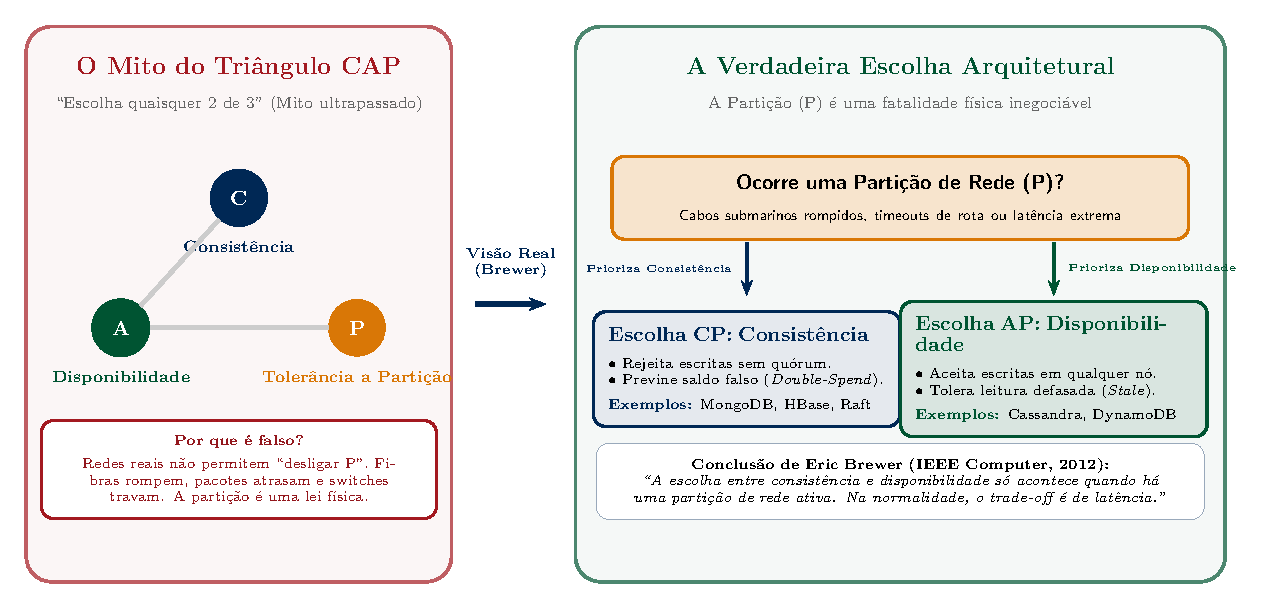
\includegraphics[width=13.6cm,height=4.8cm,keepaspectratio]{figuras/fig_cap_realidade.pdf}%
  }\par
  \vspace{0.15cm}
  \centering
  {\footnotesize \textbf{Regra de Ouro:} \textcolor{ScoutBlue}{Em sistemas distribuídos, a partição é inevitável. Sua única escolha é como agir durante a falha: CP ou AP.}}
\end{frame}

% ------------------------------------------------------------------------------
\twocolframe[title={A Regra de Quórum em Clusters de $N$ Nós},leftcol=7cm,rightcol=7cm]{%
  \alert{A Matemática da Maioria Absoluta}\par
  \itemseps[topsepi=2mm,itemsepi=3mm,labelsep=2mm,leftmargini=4mm]
  \begin{itemize}
    \item Para evitar que duas partes isoladas do cluster gravem dados conflitantes (\textit{Split-Brain}), usa-se o conceito de \textbf{Quórum}:
    \item $$\text{Quórum Mínimo} = \left\lfloor \frac{N}{2} \right\rfloor + 1$$
    \item Onde $N$ é o número total de nós votantes do cluster.
    \item Para $N = 3$ nós: Quórum = $1 + 1 = \mathbf{2 \text{ nós}}$.
    \item Para $N = 5$ nós: Quórum = $2 + 1 = \mathbf{3 \text{ nós}}$.
  \end{itemize}
}{%
  \alert{Por que o Número de Nós deve ser Ímpar?}\par
  \itemseps[topsepi=2mm,itemsepi=3mm,labelsep=2mm,leftmargini=4mm]
  \begin{itemize}
    \item Se tivermos $N = 4$ nós e a rede dividir ao meio (2 e 2), \textbf{nenhum lado tem maioria}! O cluster inteiro para.
    \item Com nós ímpares ($3, 5, 7$), qualquer divisão binária garante que \textbf{apenas um lado} terá a maioria estrita.
    \item O lado maioritário continua operando com segurança. O lado minoritário entra em modo de proteção.
  \end{itemize}
}

% ------------------------------------------------------------------------------
\begin{frame}{Anatomia do Quórum e Partição de Rede (Split-Brain)}
  \vspace{-0.3cm}
  \makebox[\linewidth][c]{%
    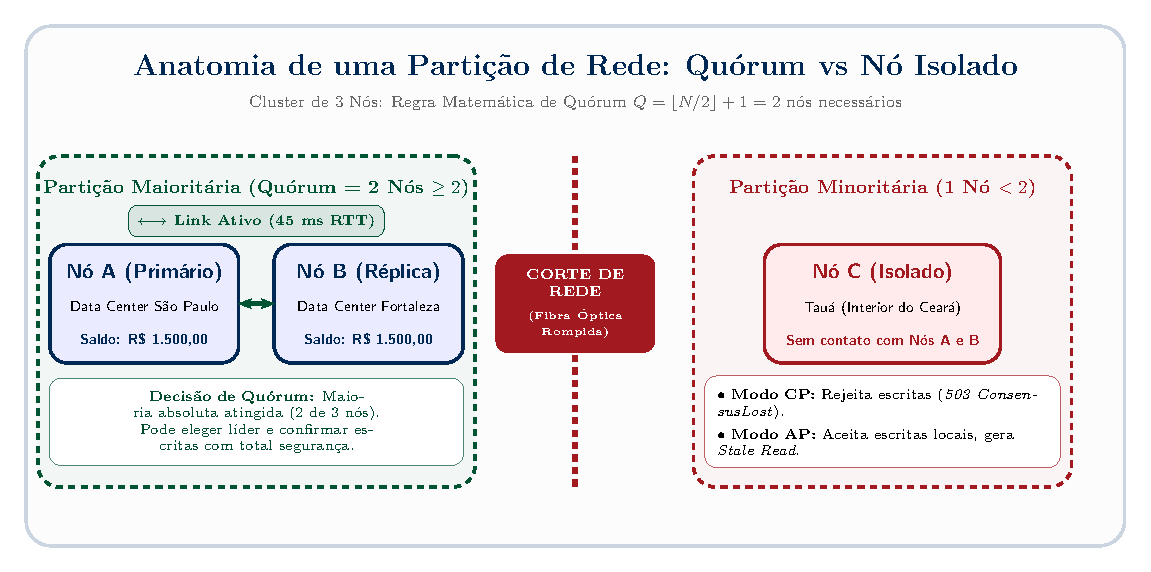
\includegraphics[width=13.6cm,height=4.8cm,keepaspectratio]{figuras/fig_cluster_split_brain.pdf}%
  }\par
  \vspace{0.15cm}
  \centering
  {\footnotesize \textbf{Comportamento:} \textcolor{ScoutBlue}{O lado maioritário (A e B) mantém o quórum de escrita. O nó isolado C deve rejeitar escritas em CP ou aceitar divergência em AP.}}
\end{frame}

% ------------------------------------------------------------------------------
\twocolframe[title={Classificação CAP dos Principais Bancos de Dados},leftcol=7cm,rightcol=7cm]{%
  \alert{Bancos do Tipo CP (Consistência Estrita)}\par
  \itemseps[topsepi=2mm,itemsepi=3mm,labelsep=2mm,leftmargini=4mm]
  \begin{itemize}
    \item \textbf{MongoDB (padrão):} Usa conjuntos de réplicas (\textit{Replica Sets}). Se o primário for isolado da maioria, ele é destituído e recusa escritas.
    \item \textbf{Apache HBase / Bigtable:} Foco absoluto em consistência via ZooKeeper/Raft.
    \item \textbf{Redis (modo Cluster com Quórum):} Rejeita escritas em partições sem mestre válido.
  \end{itemize}
}{%
  \alert{Bancos do Tipo AP (Alta Disponibilidade)}\par
  \itemseps[topsepi=2mm,itemsepi=3mm,labelsep=2mm,leftmargini=4mm]
  \begin{itemize}
    \item \textbf{Apache Cassandra:} Arquitetura \textit{masterless} (todos os nós são iguais). Permite escrita em qualquer nó disponível.
    \item \textbf{Amazon DynamoDB:} Criado especificamente para nunca recusar o carrinho de compras.
    \item \textbf{CouchDB:} Projetado para funcionar offline e sincronizar via HTTP quando a conexão voltar.
  \end{itemize}
}

\changecolours{ScoutNavy}
\section{O Teorema PACELC}

% ------------------------------------------------------------------------------
\twocolframe[title={Por que o Teorema CAP é Insuficiente no Dia a Dia?},leftcol=7cm,rightcol=7cm]{%
  \alert{O Ponto Cego de Eric Brewer}\par
  \itemseps[topsepi=2mm,itemsepi=3mm,labelsep=2mm,leftmargini=4mm]
  \begin{itemize}
    \item Em 2012, o pesquisador \textbf{Daniel J. Abadi} (Yale University) publicou um artigo seminal na IEEE:
    \item \textit{``Consistency Tradeoffs in Modern Distributed Database System Design: CAP is Only Part of the Story''}.
    \item \textbf{A Pergunta Crítica:} O que acontece quando \textbf{NÃO} há partição de rede?
  \end{itemize}
}{%
  \alert{A Realidade da Nuvem Moderna}\par
  \itemseps[topsepi=2mm,itemsepi=3mm,labelsep=2mm,leftmargini=4mm]
  \begin{itemize}
    \item Em provedores de ponta (AWS, Google Cloud, Azure), o cluster opera em estado normal durante \textbf{99,99\% do tempo}!
    \item O CAP é completamente mudo sobre o comportamento do sistema durante 99,99\% da sua vida útil.
    \item Mesmo sem falha de rede, existe um dilema feroz entre \textbf{Velocidade (Latência)} e \textbf{Coerência (Consistência)}.
  \end{itemize}
}

% ------------------------------------------------------------------------------
\twocolframe[title={A Formulação Mnemônica do Teorema PACELC},leftcol=7cm,rightcol=7cm]{%
  \alert{A Equação Arquitetural de Abadi}\par
  \vspace{0.2cm}
  {\small \textbf{Se houver Partição de Rede (\alert{P}):}}
  \begin{itemize}
    \item Escolha entre Disponibilidade (\textbf{\color{ScoutGreen}A}) ou Consistência (\textbf{\color{ScoutNavy}C}).
  \end{itemize}
  \vspace{0.2cm}
  {\small \textbf{Senão (\alert{Else - E}) em Operação Normal:}}
  \begin{itemize}
    \item Escolha entre Baixa Latência (\textbf{\color{ScoutBlue}L}) ou Consistência (\textbf{\color{ScoutNavy}C}).
  \end{itemize}
}{%
  \alert{As 4 Combinações Possíveis}\par
  \itemseps[topsepi=1.5mm,itemsepi=2.5mm,labelsep=2mm,leftmargini=4mm]
  \begin{itemize}
    \item \textbf{PA/EL:} Prioriza alta disponibilidade na partição e latência ultrabaixa no dia a dia (\textit{Cassandra, DynamoDB}).
    \item \textbf{PC/EC:} Prioriza consistência sempre, pagando o custo de esperar confirmações síncronas (\textit{MongoDB com maioria, RDBMS}).
    \item \textbf{PC/EL:} Consistente na partição, mas otimizado para baixa latência local no dia a dia (\textit{Redis, MongoDB w=1}).
  \end{itemize}
}

% ------------------------------------------------------------------------------
\begin{frame}{A Árvore Decisória Completa do Teorema PACELC}
  \vspace{-0.3cm}
  \makebox[\linewidth][c]{%
    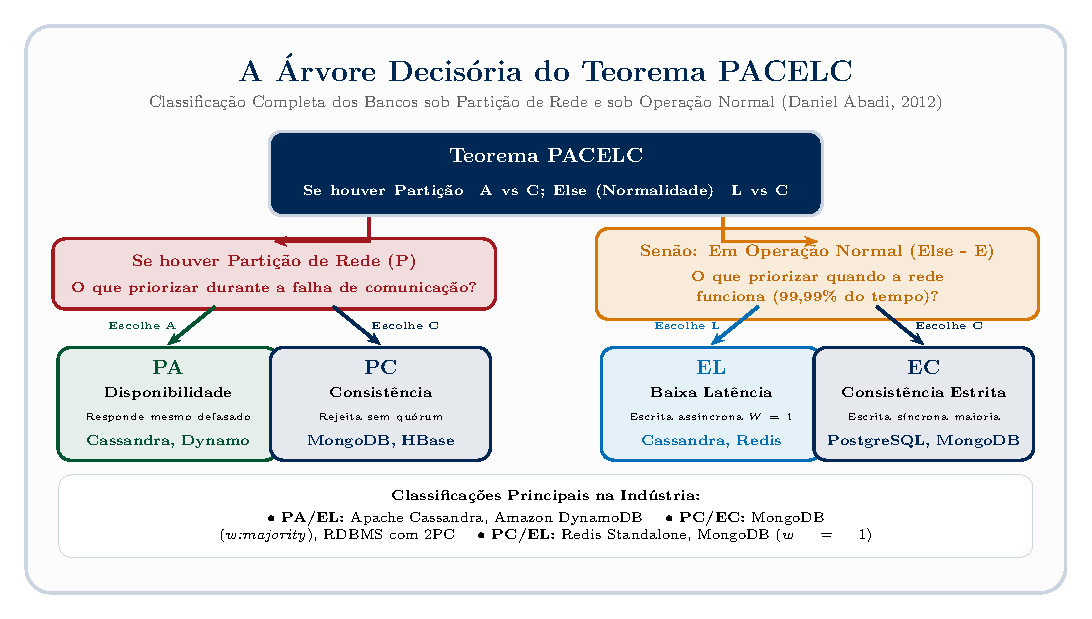
\includegraphics[width=14.0cm,height=4.8cm,keepaspectratio]{figuras/fig_pacelc_arvore.pdf}%
  }\par
  \vspace{0.15cm}
  \centering
  {\footnotesize \textbf{Visão Prática:} \textcolor{ScoutNavy}{O Teorema PACELC mapeia o comportamento do banco tanto na crise (P) quanto no estado normal (Else).}}
\end{frame}

% ------------------------------------------------------------------------------
\twocolframe[title={Exemplo Analítico: O Custo Físico da Consistência},leftcol=7cm,rightcol=7cm]{%
  \alert{Cenário de Negócio Pareado}\par
  \itemseps[topsepi=1.5mm,itemsepi=2.5mm,labelsep=2mm,leftmargini=4mm]
  \begin{itemize}
    \item Cluster com 3 nós em data centers distintos:
    \item Nó 1 (Local): $RTT_1 = 1{,}5 \text{ ms}$ (rack local).
    \item Nó 2 (Fortaleza): $RTT_2 = 45{,}0 \text{ ms}$ (regional).
    \item Nó 3 (Tauá): $RTT_3 = 58{,}0 \text{ ms}$ (interior).
    \item $RTT$ (\textit{Round-Trip Time}): tempo de ida e volta.
  \end{itemize}
}{%
  \alert{Cálculo Analítico de Latência}\par
  \itemseps[topsepi=1.5mm,itemsepi=2.5mm,labelsep=2mm,leftmargini=4mm]
  \begin{itemize}
    \item \textbf{Estratégia PA/EL (Escrita Local $W=1$):}
      $$T_{\text{EL}} = RTT_1 + 0{,}3 = \mathbf{1{,}8\text{ ms}}$$
    \item \textbf{Estratégia PC/EC (Escrita Síncrona Maioria):}
      $$T_{\text{EC}} = \max_i(RTT_i) + 2{,}0 = \mathbf{60{,}0\text{ ms}}$$
    \item \textbf{Trade-off Físico:} A consistência estrita custa $\approx \mathbf{33{,}3\times}$ mais tempo de resposta!
  \end{itemize}
}

% ------------------------------------------------------------------------------
\begin{frame}[fragile]{Demonstração Pareada em Python: Simulação PACELC}
\vspace{-0.3cm}
\begin{lstlisting}
# RTT = Round-Trip Time em milissegundos
rtt_local = 1.5; rtt_fortaleza = 45.0; rtt_taua = 58.0

# PA/EL: Confirmacao imediata no primario local (W=1)
tempo_el = rtt_local + 0.3

# PC/EC: Confirmacao sincrona aguardando quorum
tempo_ec = max(rtt_local, rtt_fortaleza, rtt_taua) + 2.0

print(f"Latencia PC/EC (Consistencia Estrita) : {tempo_ec:.1f} ms")
print(f"Latencia PA/EL (Baixa Latencia W=1)   : {tempo_el:.1f} ms")
print(f"Aceleracao no modelo EL               : {tempo_ec/tempo_el:.1f}x mais rapido!")
\end{lstlisting}
\vspace{-0.1cm}
\centering
{\scriptsize \textcolor{ScoutNavy}{\textbf{Tomada de Decisão:}} Para IoT/curtidas, escolha \textbf{EL}. Para financeiro, use \textbf{EC}.}
\end{frame}

\changecolours{ScoutGreen}
\section{Duelo de Paradigmas: ACID vs BASE}

% ------------------------------------------------------------------------------
\twocolframe[title={O Paradigma ACID: Filosofia Pessimista \& Travas},leftcol=7cm,rightcol=7cm]{%
  \alert{Origem: Jim Gray (VLDB, 1981)}\par
  \itemseps[topsepi=1.5mm,itemsepi=2.5mm,labelsep=2mm,leftmargini=4mm]
  \begin{itemize}
    \item Padrão ouro dos sistemas relacionais tradicionais (RDBMS):
    \item \textbf{Atomicidade:} A transação é indivisível (tudo ou nada).
    \item \textbf{Consistência:} Regras de negócio e chaves sempre válidas.
    \item \textbf{Isolamento:} Transações simultâneas não interferem.
    \item \textbf{Durabilidade:} Persistência permanente após commit.
  \end{itemize}
}{%
  \alert{O Gargalo da Abordagem Pessimista}\par
  \itemseps[topsepi=2mm,itemsepi=3mm,labelsep=2mm,leftmargini=4mm]
  \begin{itemize}
    \item O isolamento estrito exige \textbf{travas de leitura e escrita} (\textit{Locks}) e protocolos como \textbf{2PC} (\textit{Two-Phase Commit}).
    \item Sob concorrência massiva, travas geram filas e \textit{deadlocks}.
    \item \textbf{Filosofia:} \textit{``Prefiro travar a requisição a correr o risco de gravar um dado imperfeito.''}
  \end{itemize}
}

% ------------------------------------------------------------------------------
\twocolframe[title={O Paradigma BASE: Filosofia Otimista \& Alta Escala},leftcol=7cm,rightcol=7cm]{%
  \alert{Origem: Werner Vogels \& Dan Pritchett}\par
  \itemseps[topsepi=1.5mm,itemsepi=2.5mm,labelsep=2mm,leftmargini=4mm]
  \begin{itemize}
    \item Criado para sustentar as gigantes da Web (Amazon, Google):
    \item \textbf{BA -- Basically Available:} O sistema continua respondendo mesmo com falhas parciais em nós.
    \item \textbf{S -- Soft State:} O estado dos dados pode mudar com o tempo mesmo sem nova requisição externa.
    \item \textbf{E -- Eventual Consistency:} Réplicas convergem assincronamente para o mesmo valor com o tempo.
  \end{itemize}
}{%
  \alert{A Vantagem da Abordagem Otimista}\par
  \itemseps[topsepi=2mm,itemsepi=3mm,labelsep=2mm,leftmargini=4mm]
  \begin{itemize}
    \item Elimina completamente as travas distribuídas bloqueantes.
    \item Permite vazão de centenas de milhares de escritas por segundo.
    \item \textbf{Filosofia:} \textit{``Prefiro responder em milissegundos e reconciliar os dados assincronamente em segundo plano.''}
  \end{itemize}
}

% ------------------------------------------------------------------------------
\begin{frame}{Duelo dos Paradigmas: ACID vs. BASE Lado a Lado}
  \vspace{-0.3cm}
  \makebox[\linewidth][c]{%
    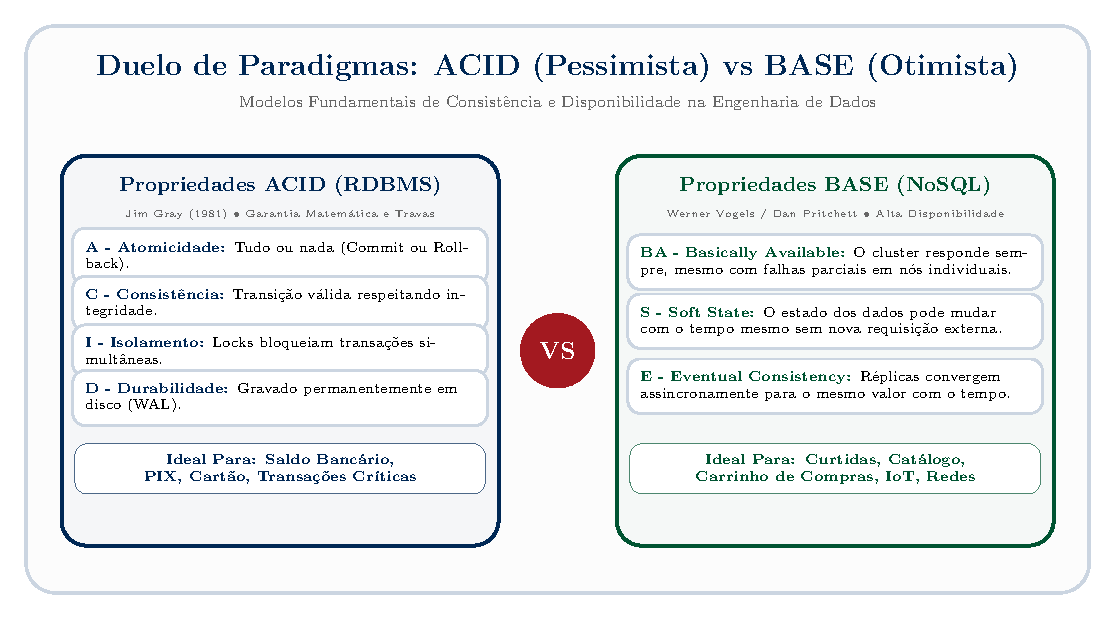
\includegraphics[width=14.0cm,height=4.8cm,keepaspectratio]{figuras/fig_acid_vs_base.pdf}%
  }\par
  \vspace{0.15cm}
  \centering
  {\footnotesize \textbf{Diretriz Arquitetural:} \textcolor{ScoutGreen}{Não existe modelo superior. O bom engenheiro de software escolhe o paradigma de acordo com o domínio de negócio.}}
\end{frame}

% ------------------------------------------------------------------------------
\twocolframe[title={Como Funciona a Consistência Eventual na Prática?},leftcol=7cm,rightcol=7cm]{%
  \alert{O Algoritmo Last-Write-Wins (LWW)}\par
  \itemseps[topsepi=2mm,itemsepi=3mm,labelsep=2mm,leftmargini=4mm]
  \begin{itemize}
    \item Cada escrita recebe um carimbo de tempo físico (\textit{timestamp}).
    \item A versão com maior carimbo sobrescreve versões anteriores.
    \item \textbf{Risco Real:} Desvios de relógio (\textit{Clock Drift}) entre servidores podem descartar escritas legítimas.
  \end{itemize}
}{%
  \alert{Vetores de Versão (Vector Clocks)}\par
  \itemseps[topsepi=2mm,itemsepi=3mm,labelsep=2mm,leftmargini=4mm]
  \begin{itemize}
    \item Cada nó mantém contadores lógicos por registro.
    \item Identifica se uma alteração foi causal ou concorrente.
    \item \textbf{Caso Real (Amazon Dynamo):} O carrinho de compras une itens conflitantes em vez de apagar qualquer um!
  \end{itemize}
}

% ------------------------------------------------------------------------------
\begin{frame}{Matriz Decisória de Negócio: Onde Aplicar Cada Paradigma}
  \vspace{-0.2cm}
  \centering
  \resizebox{0.95\textwidth}{!}{%
  \begin{tabular}{p{4.0cm}p{2.5cm}p{7.5cm}}
    \toprule
    \textbf{Domínio de Negócio} & \textbf{Paradigma} & \textbf{Justificativa Arquitetural} \\
    \midrule
    \textbf{Transferência PIX} & \textcolor{ScoutNavy}{\textbf{ACID / CP}} & O saldo não tolera inconsistência. Gasto duplo gera rombo financeiro. \\
    \addlinespace
    \textbf{Curtidas no TikTok} & \textcolor{ScoutGreen}{\textbf{BASE / AP}} & Perder pequenas contagens em milhões de visualizações é aceitável. \\
    \addlinespace
    \textbf{Carrinho de Compras} & \textcolor{ScoutGreen}{\textbf{BASE / AP}} & Rejeitar o cliente perde a venda. Melhor reconciliar itens depois. \\
    \addlinespace
    \textbf{Vagas SISU / Concursos} & \textcolor{ScoutNavy}{\textbf{ACID / CP}} & Disputas por fração de segundo exigem isolamento estrito. \\
    \bottomrule
  \end{tabular}%
  }
\end{frame}

\changecolours{ScoutRed}
\section{Taxonomia NoSQL \& Prática Hands-On}

% ------------------------------------------------------------------------------
\twocolframe[title={Os 4 Modelos NoSQL \& Bancos Vetoriais},leftcol=7cm,rightcol=7cm]{%
  \alert{Modelos Orientados a Agregados}\par
  \itemseps[topsepi=1.5mm,itemsepi=2.5mm,labelsep=2mm,leftmargini=4mm]
  \begin{itemize}
    \item \textbf{Chave-Valor (Redis, DynamoDB):} Dicionários gigantes em memória. Complexidade $O(1)$. Foco em cache e latência (\textbf{PA/EL} ou \textbf{PC/EL}).
    \item \textbf{Documentos (MongoDB, Couchbase):} JSON/BSON com esquemas flexíveis e aninhamento. Foco em aplicações web e catálogos (\textbf{PC/EC}).
    \item \textbf{Família de Colunas (Cassandra, ScyllaDB):} Colunas esparsas distribuídas em anel \textit{masterless}. Escrita massiva (\textbf{PA/EL}).
  \end{itemize}
}{%
  \alert{Grafos \& Bancos Vetoriais}\par
  \itemseps[topsepi=1.5mm,itemsepi=2.5mm,labelsep=2mm,leftmargini=4mm]
  \begin{itemize}
    \item \textbf{Orientados a Grafos (Neo4j):} Foco na riqueza de relacionamentos e travessia rápida de caminhos (\textbf{PC/EC}).
    \item \textbf{Bancos Vetoriais (ChromaDB, Pinecone):} Vetores de alta dimensão (*embeddings*) para busca semântica e IA Generativa (RAG).
  \end{itemize}
}

% ------------------------------------------------------------------------------
\begin{frame}{Taxonomia NoSQL na Matriz CAP / PACELC}
  \vspace{-0.3cm}
  \makebox[\linewidth][c]{%
    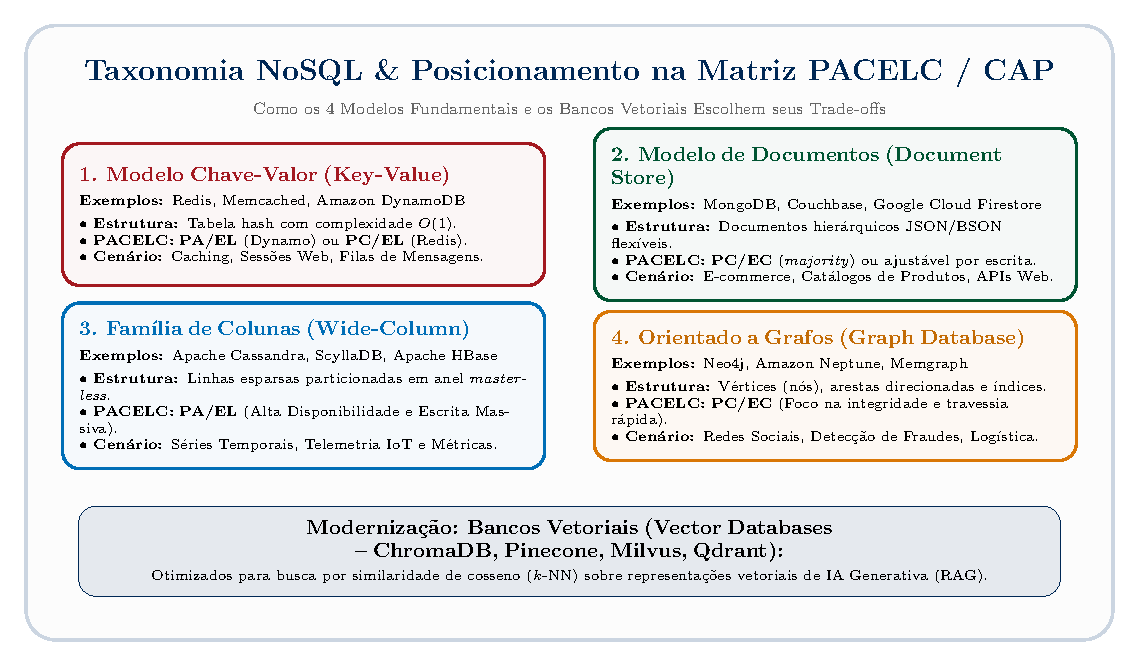
\includegraphics[width=14.0cm,height=4.8cm,keepaspectratio]{figuras/fig_taxonomia_4_modelos.pdf}%
  }\par
  \vspace{0.15cm}
  \centering
  {\footnotesize \textbf{Síntese Arquitetural:} \textcolor{ScoutRed}{Cada modelo NoSQL foi desenhado para resolver um tipo específico de acesso e trade-off.}}
\end{frame}

% ------------------------------------------------------------------------------
\begin{frame}[fragile]{MongoDB Prático: Níveis de Garantia de Escrita (Write Concern)}
\vspace{-0.2cm}
\alert{Ajustando o Teorema PACELC diretamente no código de aplicação:}\par
\vspace{0.1cm}
\begin{lstlisting}
// 1. Alta Performance / Baixa Latencia (Modo PA/EL):
db.sensores.insertOne(
  { sensor: "TAU-01", temp: 31.2 },
  { writeConcern: { w: 1, wtimeout: 1000 } }
);

// 2. Alta Seguranca e Consistencia Financeira (Modo PC/EC):
db.transferencias.insertOne(
  { de: "CTA-100", para: "CTA-200", valor: 1500.00 },
  { writeConcern: { w: "majority", j: true, wtimeout: 5000 } }
);
\end{lstlisting}
\vspace{-0.1cm}
\centering
{\scriptsize \textbf{Nota de Engenharia:} O parâmetro \texttt{w: "majority"} impede que alterações sejam revertidas por eleições de novo líder.}
\end{frame}

% ------------------------------------------------------------------------------
\begin{frame}[fragile]{MongoDB Prático: Níveis de Isolamento de Leitura (Read Concern)}
\vspace{-0.2cm}
\alert{Controlando se sua consulta pode ou não ler dados defasados (Stale Reads):}\par
\vspace{0.1cm}
\begin{lstlisting}
// 1. Leitura Local (Rapida, mas com risco de Stale Read):
db.pedidos.find({ status: "pendente" }).readConcern("local");

// 2. Leitura com Quorum Garantido (Majority Read Concern):
db.pedidos.find({ id_pedido: "PED-2026-09" }).readConcern("majority");

// 3. Leitura Linearizavel (Linearizable):
db.contas.find({ id_cliente: 42 }).readConcern("linearizable");
\end{lstlisting}
\end{frame}

% ------------------------------------------------------------------------------
\twocolframe[title={Roteiro do Laboratório Hands-On no Terminal},leftcol=7cm,rightcol=7cm]{%
  \alert{O Script Didático da Aula}\par
  \itemseps[topsepi=2mm,itemsepi=3mm,labelsep=2mm,leftmargini=4mm]
  \begin{itemize}
    \item Desenvolvido especificamente para esta aula: \texttt{demonstracao\_aula02.py}.
    \item Simula um cluster de 3 nós com injeção de rompimento de rede em tempo real.
    \item Demonstra na prática:
      \begin{itemize}
        \item Bloqueio de escritas sem quórum (CP);
        \item Escrita local e leitura defasada (AP);
        \item Reconciliação via \textit{Last-Write-Wins}.
      \end{itemize}
  \end{itemize}
}{%
  \alert{Como Executar no Laboratório}\par
  \itemseps[topsepi=2mm,itemsepi=3mm,labelsep=2mm,leftmargini=4mm]
  \begin{itemize}
    \item Abra o terminal na pasta da aula e execute:
    \item \texttt{python3 codigo/demonstracao\_aula02.py}
    \item Navegue pelo menu interativo (opções 1 a 5).
    \item Também disponível como Jupyter Notebook interativo:
    \item \texttt{codigo/demonstracao\_aula02.ipynb}
  \end{itemize}
}

% ------------------------------------------------------------------------------
\twocolframe[title={Próximo Encontro \& Atividades de Fixação},leftcol=7cm,rightcol=7cm]{%
  \alert{Sábado Letivo (10/10/2026) -- Aula 03}\par
  \itemseps[topsepi=2mm,itemsepi=3mm,labelsep=2mm,leftmargini=4mm]
  \begin{itemize}
    \item \textbf{Atenção:} Conforme o cronograma pedagógico, sábado letivo \textbf{não tem conteúdo novo}.
    \item \textbf{Oficina Prática de DevOps:} Orquestração com Docker e Docker Compose para subir instâncias de Redis e MongoDB em segundos.
    \item Resolução assistida da Lista 1 no laboratório.
  \end{itemize}
}{%
  \alert{Lista de Exercícios 1 (Bloco 2)}\par
  \itemseps[topsepi=2mm,itemsepi=3mm,labelsep=2mm,leftmargini=4mm]
  \begin{itemize}
    \item Responder às questões 7 a 12 no \texttt{README.md} da Aula 02:
      \begin{itemize}
        \item Análise de partição em 3 e 4 nós;
        \item Trade-offs de Latência vs Consistência no PACELC;
        \item Comparação de cenários do mundo real (PIX vs TikTok);
        \item Uso de Write Concern no MongoDB.
      \end{itemize}
  \end{itemize}
}


% ------------------------------------------------------------------------------
% Encerramento
% ------------------------------------------------------------------------------
\changecolours[inverse]{ScoutGreen}
\begin{frame}[plain]
  \vspace{2cm}
  \centering
  {\Huge \textbf{Dúvidas \& Discussão}}\par
  \vspace{0.8cm}
  {\large IFCE Campus Tauá -- ADS16}\par
  \vspace{0.3cm}
  {\small reginaldo.fernandes@ifce.edu.br}
\end{frame}

\end{document}
